% Options for packages loaded elsewhere
\PassOptionsToPackage{unicode}{hyperref}
\PassOptionsToPackage{hyphens}{url}
\PassOptionsToPackage{dvipsnames,svgnames,x11names}{xcolor}
%
\documentclass[
  letterpaper,
  DIV=11,
  numbers=noendperiod]{scrartcl}

\usepackage{amsmath,amssymb}
\usepackage{iftex}
\ifPDFTeX
  \usepackage[T1]{fontenc}
  \usepackage[utf8]{inputenc}
  \usepackage{textcomp} % provide euro and other symbols
\else % if luatex or xetex
  \usepackage{unicode-math}
  \defaultfontfeatures{Scale=MatchLowercase}
  \defaultfontfeatures[\rmfamily]{Ligatures=TeX,Scale=1}
\fi
\usepackage{lmodern}
\ifPDFTeX\else  
    % xetex/luatex font selection
\fi
% Use upquote if available, for straight quotes in verbatim environments
\IfFileExists{upquote.sty}{\usepackage{upquote}}{}
\IfFileExists{microtype.sty}{% use microtype if available
  \usepackage[]{microtype}
  \UseMicrotypeSet[protrusion]{basicmath} % disable protrusion for tt fonts
}{}
\makeatletter
\@ifundefined{KOMAClassName}{% if non-KOMA class
  \IfFileExists{parskip.sty}{%
    \usepackage{parskip}
  }{% else
    \setlength{\parindent}{0pt}
    \setlength{\parskip}{6pt plus 2pt minus 1pt}}
}{% if KOMA class
  \KOMAoptions{parskip=half}}
\makeatother
\usepackage{xcolor}
\setlength{\emergencystretch}{3em} % prevent overfull lines
\setcounter{secnumdepth}{-\maxdimen} % remove section numbering
% Make \paragraph and \subparagraph free-standing
\ifx\paragraph\undefined\else
  \let\oldparagraph\paragraph
  \renewcommand{\paragraph}[1]{\oldparagraph{#1}\mbox{}}
\fi
\ifx\subparagraph\undefined\else
  \let\oldsubparagraph\subparagraph
  \renewcommand{\subparagraph}[1]{\oldsubparagraph{#1}\mbox{}}
\fi

\usepackage{color}
\usepackage{fancyvrb}
\newcommand{\VerbBar}{|}
\newcommand{\VERB}{\Verb[commandchars=\\\{\}]}
\DefineVerbatimEnvironment{Highlighting}{Verbatim}{commandchars=\\\{\}}
% Add ',fontsize=\small' for more characters per line
\usepackage{framed}
\definecolor{shadecolor}{RGB}{241,243,245}
\newenvironment{Shaded}{\begin{snugshade}}{\end{snugshade}}
\newcommand{\AlertTok}[1]{\textcolor[rgb]{0.68,0.00,0.00}{#1}}
\newcommand{\AnnotationTok}[1]{\textcolor[rgb]{0.37,0.37,0.37}{#1}}
\newcommand{\AttributeTok}[1]{\textcolor[rgb]{0.40,0.45,0.13}{#1}}
\newcommand{\BaseNTok}[1]{\textcolor[rgb]{0.68,0.00,0.00}{#1}}
\newcommand{\BuiltInTok}[1]{\textcolor[rgb]{0.00,0.23,0.31}{#1}}
\newcommand{\CharTok}[1]{\textcolor[rgb]{0.13,0.47,0.30}{#1}}
\newcommand{\CommentTok}[1]{\textcolor[rgb]{0.37,0.37,0.37}{#1}}
\newcommand{\CommentVarTok}[1]{\textcolor[rgb]{0.37,0.37,0.37}{\textit{#1}}}
\newcommand{\ConstantTok}[1]{\textcolor[rgb]{0.56,0.35,0.01}{#1}}
\newcommand{\ControlFlowTok}[1]{\textcolor[rgb]{0.00,0.23,0.31}{#1}}
\newcommand{\DataTypeTok}[1]{\textcolor[rgb]{0.68,0.00,0.00}{#1}}
\newcommand{\DecValTok}[1]{\textcolor[rgb]{0.68,0.00,0.00}{#1}}
\newcommand{\DocumentationTok}[1]{\textcolor[rgb]{0.37,0.37,0.37}{\textit{#1}}}
\newcommand{\ErrorTok}[1]{\textcolor[rgb]{0.68,0.00,0.00}{#1}}
\newcommand{\ExtensionTok}[1]{\textcolor[rgb]{0.00,0.23,0.31}{#1}}
\newcommand{\FloatTok}[1]{\textcolor[rgb]{0.68,0.00,0.00}{#1}}
\newcommand{\FunctionTok}[1]{\textcolor[rgb]{0.28,0.35,0.67}{#1}}
\newcommand{\ImportTok}[1]{\textcolor[rgb]{0.00,0.46,0.62}{#1}}
\newcommand{\InformationTok}[1]{\textcolor[rgb]{0.37,0.37,0.37}{#1}}
\newcommand{\KeywordTok}[1]{\textcolor[rgb]{0.00,0.23,0.31}{#1}}
\newcommand{\NormalTok}[1]{\textcolor[rgb]{0.00,0.23,0.31}{#1}}
\newcommand{\OperatorTok}[1]{\textcolor[rgb]{0.37,0.37,0.37}{#1}}
\newcommand{\OtherTok}[1]{\textcolor[rgb]{0.00,0.23,0.31}{#1}}
\newcommand{\PreprocessorTok}[1]{\textcolor[rgb]{0.68,0.00,0.00}{#1}}
\newcommand{\RegionMarkerTok}[1]{\textcolor[rgb]{0.00,0.23,0.31}{#1}}
\newcommand{\SpecialCharTok}[1]{\textcolor[rgb]{0.37,0.37,0.37}{#1}}
\newcommand{\SpecialStringTok}[1]{\textcolor[rgb]{0.13,0.47,0.30}{#1}}
\newcommand{\StringTok}[1]{\textcolor[rgb]{0.13,0.47,0.30}{#1}}
\newcommand{\VariableTok}[1]{\textcolor[rgb]{0.07,0.07,0.07}{#1}}
\newcommand{\VerbatimStringTok}[1]{\textcolor[rgb]{0.13,0.47,0.30}{#1}}
\newcommand{\WarningTok}[1]{\textcolor[rgb]{0.37,0.37,0.37}{\textit{#1}}}

\providecommand{\tightlist}{%
  \setlength{\itemsep}{0pt}\setlength{\parskip}{0pt}}\usepackage{longtable,booktabs,array}
\usepackage{calc} % for calculating minipage widths
% Correct order of tables after \paragraph or \subparagraph
\usepackage{etoolbox}
\makeatletter
\patchcmd\longtable{\par}{\if@noskipsec\mbox{}\fi\par}{}{}
\makeatother
% Allow footnotes in longtable head/foot
\IfFileExists{footnotehyper.sty}{\usepackage{footnotehyper}}{\usepackage{footnote}}
\makesavenoteenv{longtable}
\usepackage{graphicx}
\makeatletter
\def\maxwidth{\ifdim\Gin@nat@width>\linewidth\linewidth\else\Gin@nat@width\fi}
\def\maxheight{\ifdim\Gin@nat@height>\textheight\textheight\else\Gin@nat@height\fi}
\makeatother
% Scale images if necessary, so that they will not overflow the page
% margins by default, and it is still possible to overwrite the defaults
% using explicit options in \includegraphics[width, height, ...]{}
\setkeys{Gin}{width=\maxwidth,height=\maxheight,keepaspectratio}
% Set default figure placement to htbp
\makeatletter
\def\fps@figure{htbp}
\makeatother

\usepackage{booktabs}
\usepackage{caption}
\usepackage{longtable}
\usepackage{colortbl}
\usepackage{array}
\KOMAoption{captions}{tableheading}
\usepackage{fontspec}
\setmainfont{Times New Roman}
\renewcommand{\normalsize}{\fontsize{12}{18}\selectfont}
\makeatletter
\makeatother
\makeatletter
\makeatother
\makeatletter
\@ifpackageloaded{caption}{}{\usepackage{caption}}
\AtBeginDocument{%
\ifdefined\contentsname
  \renewcommand*\contentsname{Table of contents}
\else
  \newcommand\contentsname{Table of contents}
\fi
\ifdefined\listfigurename
  \renewcommand*\listfigurename{List of Figures}
\else
  \newcommand\listfigurename{List of Figures}
\fi
\ifdefined\listtablename
  \renewcommand*\listtablename{List of Tables}
\else
  \newcommand\listtablename{List of Tables}
\fi
\ifdefined\figurename
  \renewcommand*\figurename{Figure}
\else
  \newcommand\figurename{Figure}
\fi
\ifdefined\tablename
  \renewcommand*\tablename{Table}
\else
  \newcommand\tablename{Table}
\fi
}
\@ifpackageloaded{float}{}{\usepackage{float}}
\floatstyle{ruled}
\@ifundefined{c@chapter}{\newfloat{codelisting}{h}{lop}}{\newfloat{codelisting}{h}{lop}[chapter]}
\floatname{codelisting}{Listing}
\newcommand*\listoflistings{\listof{codelisting}{List of Listings}}
\makeatother
\makeatletter
\@ifpackageloaded{caption}{}{\usepackage{caption}}
\@ifpackageloaded{subcaption}{}{\usepackage{subcaption}}
\makeatother
\makeatletter
\@ifpackageloaded{tcolorbox}{}{\usepackage[skins,breakable]{tcolorbox}}
\makeatother
\makeatletter
\@ifundefined{shadecolor}{\definecolor{shadecolor}{rgb}{.97, .97, .97}}
\makeatother
\makeatletter
\makeatother
\makeatletter
\makeatother
\ifLuaTeX
  \usepackage{selnolig}  % disable illegal ligatures
\fi
\IfFileExists{bookmark.sty}{\usepackage{bookmark}}{\usepackage{hyperref}}
\IfFileExists{xurl.sty}{\usepackage{xurl}}{} % add URL line breaks if available
\urlstyle{same} % disable monospaced font for URLs
\hypersetup{
  pdftitle={Arbeidskrav 1 - reliabilitet og reproduserbar dataanalyse},
  colorlinks=true,
  linkcolor={blue},
  filecolor={Maroon},
  citecolor={Blue},
  urlcolor={Blue},
  pdfcreator={LaTeX via pandoc}}

\title{Arbeidskrav 1 - reliabilitet og reproduserbar dataanalyse}
\author{}
\date{}

\begin{document}
\maketitle
\ifdefined\Shaded\renewenvironment{Shaded}{\begin{tcolorbox}[frame hidden, borderline west={3pt}{0pt}{shadecolor}, enhanced, breakable, interior hidden, boxrule=0pt, sharp corners]}{\end{tcolorbox}}\fi

Dette er en studie gjennomført i emnet IDR4000, som en del av
masterprogrammet i treningsfysiologi. Hensikten med denne
oppgaven/studien er å anslå hvor pålitelig testen er ut ifra målinger
som er samlet inn i fysiologilabben. I tillegg får vi øvd på våre
ferdigheter i å gjennomføre laboratorietester. Et annet mål med oppgaven
er å bruke programvaren R som et verktøy for reproduserbar
datavitenskap.

Vi rekrutterte åtte personer til å gjennomføre en styrketest, samt noen
utholdenhetstester på sykkel. Testene ble gjennomført to ganger, på to
separate dager.

\hypertarget{metode}{%
\subsection{Metode}\label{metode}}

\hypertarget{forsuxf8kspersonene}{%
\subsubsection{Forsøkspersonene}\label{forsuxf8kspersonene}}

Syv mannlige deltaker ble rekruttert til prosjektet (alder = 25,7 ± 7
år, vekt = 75,7 ± 10,8 kg, høyde = 181,3 ± 6,7 cm). Alle deltakerne
trener regelmessig, men erfaring med trening på sykkel varierte innad i
gruppa. Det var ingen av deltakerne som hadde noe særlig erfaring med
sykkeltestene vi gjennomførte.

\begin{Shaded}
\begin{Highlighting}[]
\NormalTok{reablitet2 }\SpecialCharTok{|\textgreater{}} 
  \FunctionTok{filter}\NormalTok{(timepoint }\SpecialCharTok{==} \StringTok{"t1"}\NormalTok{) }\SpecialCharTok{|\textgreater{}} 
  \FunctionTok{select}\NormalTok{(timepoint, age}\SpecialCharTok{:}\NormalTok{bodymass, vo2.rel.max, w.max) }\SpecialCharTok{|\textgreater{}} 
  \FunctionTok{pivot\_longer}\NormalTok{(}\AttributeTok{cols =} \SpecialCharTok{!}\NormalTok{timepoint,}
               \AttributeTok{names\_to =} \StringTok{"variabler"}\NormalTok{, }
               \AttributeTok{values\_to =} \StringTok{"verdier"}\NormalTok{) }\SpecialCharTok{|\textgreater{}} 
  \FunctionTok{mutate}\NormalTok{(}\AttributeTok{variabel =} \FunctionTok{factor}\NormalTok{(variabler, }
                           \AttributeTok{levels =} \FunctionTok{c}\NormalTok{(}\StringTok{"age"}\NormalTok{, }
                                      \StringTok{"bodyheight"}\NormalTok{, }
                                      \StringTok{"bodymass"}\NormalTok{, }
                                      \StringTok{"vo2.rel.max"}\NormalTok{, }
                                      \StringTok{"w.max"}\NormalTok{), }
                           \AttributeTok{labels =} \FunctionTok{c}\NormalTok{(}\StringTok{"Alder (år)"}\NormalTok{, }
                                      \StringTok{"Høyde (cm)"}\NormalTok{, }
                                      \StringTok{"Vekt (kg)"}\NormalTok{, }
                                      \StringTok{"VO2maks"}\NormalTok{, }
                                      \StringTok{"Wmaks"}\NormalTok{)))  }\SpecialCharTok{|\textgreater{}} 
  
  \FunctionTok{summarise}\NormalTok{(}\AttributeTok{m =} \FunctionTok{mean}\NormalTok{(verdier), }
            \AttributeTok{s =} \FunctionTok{sd}\NormalTok{(verdier), }
            \AttributeTok{.by =}\NormalTok{ variabel) }\SpecialCharTok{|\textgreater{}} 
  \FunctionTok{gt}\NormalTok{() }\SpecialCharTok{|\textgreater{}} 
  \FunctionTok{fmt\_number}\NormalTok{(}\AttributeTok{decimals =} \DecValTok{2}\NormalTok{) }\SpecialCharTok{|\textgreater{}} 
  \FunctionTok{cols\_merge}\NormalTok{(}\AttributeTok{columns =} \FunctionTok{c}\NormalTok{(m, s), }
             \AttributeTok{pattern =} \StringTok{"\{1\} \&plusmn; \{2\}"}\NormalTok{) }\SpecialCharTok{|\textgreater{}} 
  \FunctionTok{cols\_label}\NormalTok{(}\AttributeTok{m =}\StringTok{""}\NormalTok{) }\SpecialCharTok{|\textgreater{}} 
  \FunctionTok{tab\_footnote}\NormalTok{(}\AttributeTok{footnote =} \FunctionTok{md}\NormalTok{(}\StringTok{"*Dataene er presentert som gjennomsnitt \&plusmn; }
\StringTok{                             standardavvik.*"}\NormalTok{)) }\SpecialCharTok{|\textgreater{}} 
  \FunctionTok{cols\_width}\NormalTok{(}\AttributeTok{columns =} \FunctionTok{everything}\NormalTok{() }\SpecialCharTok{\textasciitilde{}} \FunctionTok{px}\NormalTok{(}\DecValTok{120}\NormalTok{)) }\SpecialCharTok{|\textgreater{}} 
  \FunctionTok{tab\_header}\NormalTok{(}\StringTok{"Karakteristikker av forsøkspersonene basert på første test"}\NormalTok{) }
\end{Highlighting}
\end{Shaded}

\setlength{\LTpost}{0mm}
\begin{longtable*}{>{\centering\arraybackslash}p{120px}>{\raggedleft\arraybackslash}p{120px}}
\caption*{
{\large Karakteristikker av forsøkspersonene basert på første test}
} \\ 
\toprule
variabel &  \\ 
\midrule\addlinespace[2.5pt]
Alder (år) & $25.71$ &plusmn; $3.55$ \\ 
Høyde (cm) & $181.29$ &plusmn; $4.57$ \\ 
Vekt (kg) & $75.66$ &plusmn; $7.37$ \\ 
VO2maks & $66.23$ &plusmn; $7.23$ \\ 
Wmaks & $410.00$ &plusmn; $58.95$ \\ 
\bottomrule
\end{longtable*}
\begin{minipage}{\linewidth}
\emph{Dataene er presentert som gjennomsnitt ±
standardavvik.}\\
\end{minipage}

\begin{verbatim}
Warning: HTML tags found, and they will be removed.
* Set `options(gt.html_tag_check = FALSE)` to disable this check.
HTML tags found, and they will be removed.
* Set `options(gt.html_tag_check = FALSE)` to disable this check.
HTML tags found, and they will be removed.
* Set `options(gt.html_tag_check = FALSE)` to disable this check.
\end{verbatim}

\begin{longtable*}{lrrrrr}
\caption*{
{\large Gjennomsnitt for t1 og t2}
} \\ 
\toprule
Tidspunkt & Wmaks & VO2maks
(ml·kg-1·min-1) & RER & VE(l·min-1) & BF \\ 
\midrule\addlinespace[2.5pt]
t1 & $410.0$ & $66.2$ & $1.2$ & $201.6$ & $59.2$ \\ 
t2 & $404.3$ & $65.6$ & $1.2$ & $199.4$ & $58.1$ \\ 
\bottomrule
\end{longtable*}

\hypertarget{studiedesign}{%
\subsubsection{Studiedesign}\label{studiedesign}}

Prosjektets testdager bestod av fire dager. Halvparten av dem ble testet
hver dag, slik at deltakerne hadde én rolig dag mellom sine egne tester.
Testdag 1 og 2 ble gjennomført som t1, mens testdag 3 og 4 ble
gjennomført som t2. På hviledagen fikk alle deltakerne beskjed om at de
kunne trene det de selv ønsket av rolig trening. Dette for å sikre at de
var tilnærmet likt restituert før hver test. For alle deltakerne ble det
forsøkt å gjøre testdagene så identiske som mulig i form av at
forsøkspersonene fikk samme testleder på hver test (ett unntak pga.
logistiske utfordringer for testleder), likt tidspunkt på døgnet ± 2
timer, beskjed om likt måltid og til samme tid før test.

\hypertarget{kalibrering---klargjuxf8ring-til-test}{%
\subsubsection{Kalibrering - klargjøring til
test}\label{kalibrering---klargjuxf8ring-til-test}}

Før hver forsøksperson skulle starte sykkeltesten kalibrerte vi oxycon
pro og Lode Excalibur-sykkelen. Vi sjekket at luftfuktigheten og
temperaturen i rommet stemte overens med oxycon sin estimering. Videre
gjennomførte vi volumkalibrering, og sørget for at verdiene for O2 og
CO2 var godkjent (± 1 \% i forskjell, og mellom 99.0 og 101.0). ``Gas
calibration'' startet da gassflaska åpnes, og var ferdig når verdiene
for O2 og CO2 lå på en verdi mellom -1.0 og 1.0, med en feilmargin på
maksimalt 1.0. Hvis det var noe som ikke stemte, eller vi ikke fikk gode
nok målinger gjorde vi den aktuelle kalibreringen på nytt. Den siste
klargjøring av maskinen var å gjøre klart VO2-opptak i ``Mixing
Chamber''. Vi kontrollerte at det stod ``small mouthpiece'' og ``30 sek
delta time'' i vinduet, og klargjorde til opptak.

Videre var det å klargjøre sykkelen ved å stille inn riktig
sittestilling. Ved t1 ble dette gjort sammen med forsøksperson, mens ved
t2 hadde vi lagret det gamle sittestillingen og kopierte denne. Riktig
setehøyde og -lengde og styrehøyde og -lengde, samt riktig pedaltype og
krankarm ble stilt inn.

De siste forberedelsene var å klargjøre munnstykket, slange og neseklype
med teip. I tillegg til å legge inn forsøkspersonen i datamaskinen med
aktuell informasjon.

\hypertarget{testprosedyre}{%
\subsubsection{Testprosedyre}\label{testprosedyre}}

Deltakerne startet med en syv minutters lang oppvarming på ergometer
sykkel, med en gradvis økning i intensitet. Intensiteten ble styrt etter
Borgs 6-20 skala. De syklet 3 min tilsvarende opplevd anstrengelse på
11, 2 min på 13 og 2 min på 15/16 på Borgs 6-20 skala.

Del 1 styrketest: Etter oppvarming gjennomførte deltakerne en kort
styrketest, i form av knebøy power test. Den bestod av tre løft med 20
kg, tre løft med henholdsvis 30-, 60- og 75 \% av egen kroppsvekt. Målet
var å gjennomføre løftet så huritig som mulig, og kraftutviklingen ble
målt med en muscle lab hastighetsmåler. Beste forsøk på hver belastning
ble tellende. Vi går ikke noe mer inn på styrketesten, fordi det er på
sykkeltesten vi har gjort analyser.

Del 2 sykkeltester: Deltakerne gikk direkte fra styrketesten til
sykkeltestene. Her gjennomførte de en tredelt test, som først bestod av
to submaksimale drag, deretter en VO\(_{2maks}\)-test og til slutt en
Maximal Accumulated Oxygen Deficit (MAOD)-test. Testene ble gjennomført
på Lode Excalibur ergometersykkel.

Under hele sykkeltesten prøvde vi å kjøre mest mulig lik tilbakemelding
og engasjement hver gang. Det var lite tilbakemeldinger under de
submaksimale dragene, og mye engasjement og kun nødvendig informasjon
under VO\(_{2maks}\)-testen, spesielt mot slutten. Vi ga ingen
opplysninger om oksygenopptak (VO2) underveis, men de fikk vite
wattbelastning. I tillegg til at de hele tiden kunne se tråkkfrekvensen
under alle testene. Vi fikk O\(_2\)-målinger hvert 30.sek som vi noterte
ned (både på VO\(_{2maks}\)-testen og MAOD-testen), i tillegg til at vi
noterte ned watt, tråkkfrekvens, puls og lengden på de to siste testene.

\hypertarget{submaksimale-drag}{%
\paragraph{Submaksimale drag}\label{submaksimale-drag}}

Den submaksimale testen bestod av to drag på fire minutter. For seks av
deltakerne ble første belastning på testen gjennomført med en effekt (W)
på 100 W og andre belastning på 150 W, mens én deltaker syklet på 75 W
og 125 W. Tilpasningene ble gjort for å få en mer optimal test.
Forsøkspersonene syklet med neseklype og munnstykket i de siste to
minuttene av hvert drag (begynte å ta i da det hadde gått 1,5 min).
Deltakerne skulle holde en tråkkfrekvens på 90-100 rpm. Hver belastning
ble gjennomført på samme måte, og gikk direkte over i hverandre. Vi
spurte om Borgs-skala etter hvert drag. Etter dragene var det to
minutter pause der deltakerne satt helt i ro.Tråkkfrekvensen til en
bestemt deltaker ble reprodusert på alle andre submaksimale drag og
under MAOD-testen så lenge de klarte.

\hypertarget{vo_2maks-test}{%
\paragraph{\texorpdfstring{VO\(_2maks\)-test}{VO\_2maks-test}}\label{vo_2maks-test}}

VO\(_{2maks}\)-testen startet for de fleste på 200 W, og økte med 25 W
hvert minutt helt til utmattelse. For deltakeren som hadde litt lavere
effekt på de submaksimale dragene startet VO\(_{2maks}\)-testen på 150
W. Testen var ferdig da tråkkfrekvens var \textless{} 60 rpm. Det var
fri tråkkfrekvens og vi målte oksygenopptaket under hele testen. Vi
spurte om Borgs-skala rett etter VO\(_{2maks}\)-testen. Etter avsluttet
test fikk forsøkspersonen fem minutter pause. Det første minuttet etter
avsluttet test satt personen helt i ro, mens de neste fire minuttene ble
gjennomført som rolig sykling på 50 W. Valgfri tråkkfrekvens, men den
skulle være lik under pausen på t2.

\hypertarget{maod-test}{%
\paragraph{MAOD-test}\label{maod-test}}

MAOD-testens starteffekt baserte seg på VO\(_{2maks}\)-testen. Effekten
de startet på var den siste belastningen deltakeren syklet 30.sek eller
mer på under VO2maks-testen. Den belastningen som ble brukt under t1 ble
også brukt på t2 uavhengig av hvordan de presterte på
VO\(_{2maks}\)-test ved t2. Deltakerne syklet med neseklype og
munnstykket under hele testen, og startet med ``flying start'' fra 50 W.
Belastningen ble satt klart på maskinen, slik at den var klar når
testleder ga beskjed om at testen skulle starte. Deltakerne syklet så
lenge som mulig, og testen var over når tråkkfrekvensen var \textless{}
60. Vi spurte om Borgs-skala rett etter avsluttet test.

\hypertarget{tiltak-for-uxe5-sikre-god-reliabilitet}{%
\subsubsection{Tiltak for å sikre god
reliabilitet}\label{tiltak-for-uxe5-sikre-god-reliabilitet}}

For å sikre en god reliabilitet på de fysiologiske testene gjorde vi
flere tiltak for å redusere risikoen for forstyrrende variabler som kan
påvirke resultatene. For det første ble begge testene kjørt på så
nøyaktig lik måte som mulig, med en standardisert protokoll. Testene for
hver forsøksperson ble avholdt på omtrent samme tidspunkt (± 2 timer).
Vi ga også beskjed om at de bare kunne trene rolig dagen før t1, og
dagen i mellom testene. På den måten sikret vi at ingen var
treningspåvirket og forhåpentligvis likt restituert før hver test.
Deltakerne fikk også beskjed om at siste måltid før begge testene skulle
være like, og til omtrent samme tidspunkt.

Vi kjørte også samme tråkkfrekvensen ved første submaksimale
belastningstrinn og ved MAOD-testen, og dette ble kopiert ved t2. Det
var lik belastning og lengde på pause før hver MAOD-test begge dager
uansett utfall på VO\(_{2maks}\)-testen. I tillegg ble hele sykkeltesten
gjennomført sittende.

Vi valgte også å ha samme testleder for hver enkelt forsøksperson ved
både t1 og t2. Den muntlige oppmuntringen og tilbakemeldingene underveis
på testene var lik, og vi sørget for å gi like instruksjoner om
utførelsen av testene og målet med hver test.

Det ble også kjørt kalibrering av oxycon pro før hver test, og vi satte
godkjent kalibrering på volum til ± 1 \%, og godkjent kalibrering av
gass med en feilmargin på maksimalt ± 1.0 \%.

\hypertarget{datainnsamling-og--behandling}{%
\subsubsection{Datainnsamling og
-behandling}\label{datainnsamling-og--behandling}}

Etter å ha gjennomført testene samlet vi inn dataene vi skulle bruke for
å gjøre statistiske analyser. Vi noterte ned VO2 på de submaksimale
dragene, og regnet ut VO2.rel.max og VO2.max på VO2maks-testen i excel.
Samtidig noterte vi ned andre verdifulle variabler etter test, slik som
hr.max, W.max, rer.max, bf.max, VE.max, hvor lenge personen syklet, og
hvilken watt personen avsluttet på, samt opplevd anstrengelse (Borg).

Etter MAOD-testen regnet vi ut VO2.max, oksygenkravet ved belastning
under MAOD-test (L/min), det totale okysgenkravet som måtte dekkes (L),
akkumulert oksygenopptak på testene (L), akkumulert oksygengjeld og
prosent av arbeidet som ble dekket anaerobt (\%). Samtidig noterte vi
ned hvor lenge personen syklet (i sekunder), makspuls og opplevd
anstrengelse (Borg).

\hypertarget{resultater}{%
\subsubsection{Resultater}\label{resultater}}

For relativ VO\(_{2maks}\) var differansen mellom testene 0.62 ± 2.41
\(ml·kg^{-1}·min^{-1}\). Med en typisk målefeil på 1.7. I prosentvis
forskjell mellom testene var det 0.94 ± 3.65 \% for denne variabelen.

For W\(_{maks}\) og ventilasjonen er differansen mellom testene
henholdsvis 5.71 ± 13.80 W og 2.21 ± 11.42 l/min. Den typiske målefeilen
var hhv. 9.8 og 8.1, mens cv var 2.4 og 4.

Figuren under viser at det er en korrelasjon mellom effekten de har på
siste minuttet av makstesten og relativ VO\(_{2maks}\) ved begge
testene, som er å forvente.

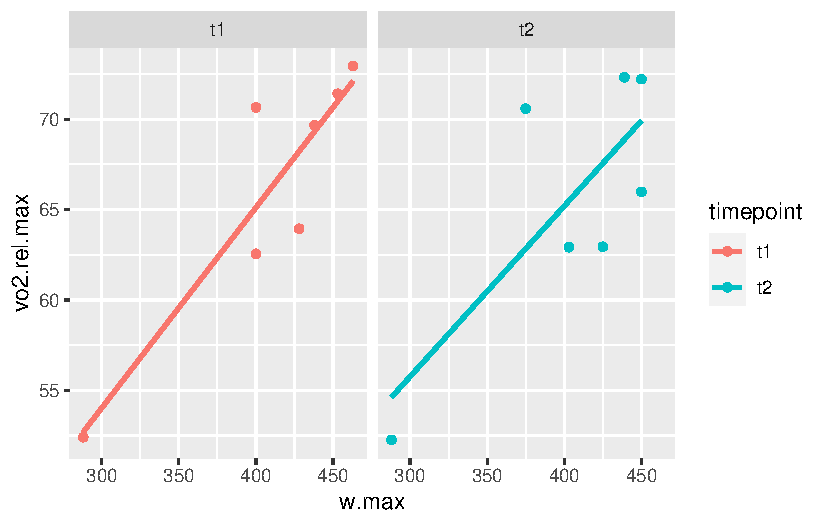
\includegraphics{Protokoll_files/figure-pdf/unnamed-chunk-5-1.pdf}



\end{document}
